\documentclass[aspectratio=169]{beamer}

\usepackage{ccicons}
\usepackage{fontspec}
\usepackage{import}
\usepackage{listings}
\usepackage{tikz}

\subimport{../}{colors.tex}

\usetikzlibrary{
  arrows,
  arrows.meta,
  automata,
  backgrounds,
  calc,
  chains,
  decorations.pathreplacing,
  fit,
  matrix,
  overlay-beamer-styles,
  positioning,
  shapes,
  tikzmark,
}
\usetikzmarklibrary{listings}

\hypersetup{
  colorlinks=true,
  urlcolor=uclablue,
}

\setbeamercolor{frametitle}{fg=primarycolor}
\setbeamercolor{structure}{fg=primarycolor}
\setbeamercolor{enumerate item}{fg=black}
\setbeamercolor{itemize item}{fg=black}
\setbeamercolor{itemize subitem}{fg=black}

\setbeamersize{text margin left=26.6mm}
\addtolength{\headsep}{2mm}

\setbeamertemplate{navigation symbols}{}
\setbeamertemplate{headline}{}
\setbeamertemplate{footline}{}
\setbeamertemplate{itemize item}{\color{black}}
\setbeamertemplate{itemize items}[circle]

\setbeamertemplate{footline}{
  \begin{tikzpicture}[remember picture,
                      overlay,
                      shift={(current page.south west)}]
    \node [black!50, inner sep=2mm, anchor=south east]
          at (current page.south east) {\footnotesize \insertframenumber};
  \end{tikzpicture}
}

\setsansfont{Overpass}[Scale=MatchLowercase]
\setmonofont{Overpass Mono}[Scale=MatchLowercase]

\makeatletter
\newcommand\version[1]{\renewcommand\@version{#1}}
\newcommand\@version{}
\def\insertversion{\@version}

\newcommand\lecturenumber[1]{\renewcommand\@lecturenumber{#1}}
\newcommand\@lecturenumber{}
\def\insertlecturenumber{\@lecturenumber}
\makeatother

\setbeamertemplate{title page}
{
  \begin{tikzpicture}[remember picture,
                      overlay,
                      shift={(current page.south west)},
                      background rectangle/.style={fill=uclablue},
                      show background rectangle]
    \node [anchor=west, align=left, inner sep=0, text=white]
          (lecturenumber) at (\paperwidth / 6, \paperheight * 3 / 4)
          {\Large Lecture \insertlecturenumber};
    \node [inner sep=0, align=left, text=white, node distance=0,
           above left=of lecturenumber, anchor=south west, yshift=2mm]
          {\Large CS 111: Operating System Principles};
    \node (title) [inner sep=0, anchor=west, align=right, text=white]
          at (\paperwidth / 6, \paperheight / 2)
          {{\bfseries \Huge \inserttitle{}}};
    \node [inner sep=0, align=right, text=white, node distance=0,
           below right=of title, anchor=north east, yshift=-1mm]
          {{\footnotesize \ttfamily \insertversion}};
    \node [inner sep=0, text=white, align=left, anchor=west]
          (author) at (\paperwidth / 6, \paperheight / 4)
          {\insertauthor};
    \node [text=white, inner sep=0, align=left, node distance=0,
           below left=of author, anchor=north west, yshift=-2mm]
          {\insertdate};
    \node [align=right, anchor=south east, inner sep=2mm, text=white]
          (license) at (\paperwidth, 0)
          {\footnotesize This  work is licensed under a
           \href{http://creativecommons.org/licenses/by-sa/4.0/}
                {\color{uclagold} Creative Commons Attribution-ShareAlike 4.0
                 International License}};
    \node [text=white, inner sep=0, align=right, node distance=0,
           above right=of license, anchor=south east, xshift=-2mm]
          {\Large \ccbysa};
  \end{tikzpicture}
}

\tikzset{
  >=Straight Barb[],
  shorten >=1pt,
  initial text=,
}

\lstset{
  basicstyle=\footnotesize\ttfamily,
}


\lecturenumber{15}
\title{Filesystems}
\version{3.0.1}
\author{Jon Eyolfson}
\date{November 18, 2021}

\begin{document}
  \begin{frame}[plain, noframenumbering]
    \titlepage
  \end{frame}

  \begin{frame}{Filesystems}
    Usual layout of a POSIX Filesystem (here: parts of FHS):
    \begin{center}
      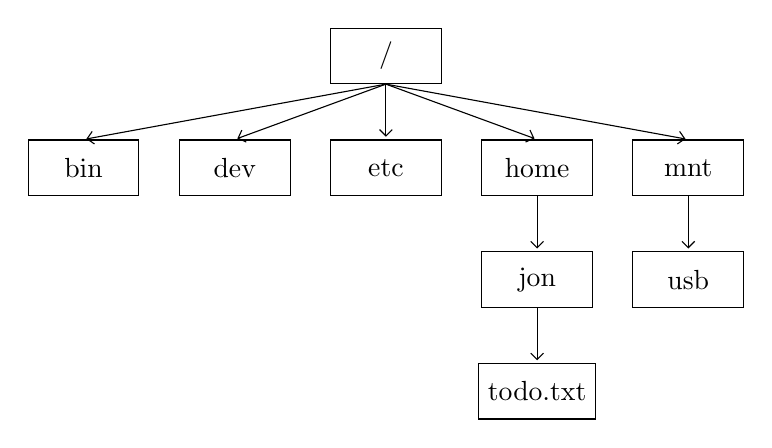
\begin{tikzpicture}[node distance=0mm and 5mm]

        \node[draw,rectangle,minimum width=40,minimum height=20] (root)  {/};
        \node[draw,rectangle,minimum width=40,minimum height=20,yshift=-20] (etc) [below=of root] {etc};
        \node[draw,rectangle,minimum width=40,minimum height=20] (dev) [left=of etc] {dev};
        \node[draw,rectangle,minimum width=40,minimum height=20] (bin) [left=of dev] {bin};
        \node[draw,rectangle,minimum width=40,minimum height=20] (home) [right=of etc] {home};
        \node[draw,rectangle,minimum width=40,minimum height=20] (mnt) [right=of home] {mnt};
    
    
        \node[draw,rectangle,minimum width=40,minimum height=20,yshift=-20] (jon) [below=of home] {jon};
        \node[draw,rectangle,minimum width=40,minimum height=20,yshift=-20] (todotxt) [below=of jon] {todo.txt};
    
        \node[draw,rectangle,minimum width=40,minimum height=20,yshift=-20] (usb) [below=of mnt] {usb};
    
        \draw[->] (root.south) -- (bin.north);
        \draw[->] (root.south) -- (dev.north);
        \draw[->] (root.south) -- (etc.north);
        \draw[->] (root.south) -- (home.north);
        \draw[->] (root.south) -- (mnt.north);
        \draw[->] (home.south) -- (jon.north);
        \draw[->] (mnt.south) -- (usb.north);
        \draw[->] (jon.south) -- (todotxt.north);
    
      \end{tikzpicture}
    \end{center}

    Working Directory: /home/jon\\

    What is the absolute and relative path to \textbf{todo.txt}? To \textbf{usb}?
  \end{frame}

  \begin{frame}{POSIX Filesystem}
    todo.txt Relative: ./todo.txt

    todo.txt Absolute: /home/jon/todo.txt

    usb Relative: ../../mnt/usb

    usb Absolute: /mnt/usb

    \vspace{2em}

    Special symbols:

    \hspace{2em} . --- Current directory
    
    \hspace{2em} .. ---  Parent directory

    \hspace{2em} $\mathsf{\sim}$ --- User's home directory (\$HOME)

    Relative paths are calculated from current working directory (\$PWD)
  \end{frame}

  \begin{frame}{You Can Access Files Sequentially or Randomly}
    Sequential access

    \vspace{2em}

    \hspace{2em} Each read advances the position inside the file

    \hspace{2em} Writes are appended and the position set to the end afterwards

    \vspace{2em}

    Random access

    \hspace{2em} Records can be read/written to the file in any order

    \hspace{2em} A specific position is required for each operation
  \end{frame}

  \begin{frame}[fragile]{POSIX Filesystem}

    \begin{lstlisting}
int open(const char *pathname, int flags, mode_t mode);

// flags can specify which operations: O_RDWR,O_WRONLY, O_RDWR
// also: O_APPEND moves the position to the end of the file initially

off_t lseek(int fd, off_t offset, int whence);

// lseek changes the position to the offset
// whence can be one of: SEEK_SET, SEEK_CUR, SEEK_END
//   set makes the offset absolute, cur and end are both relative
    \end{lstlisting}
  \end{frame}

  \begin{frame}[fragile]{Accessing Directory API}

    \begin{lstlisting}
DIR *opendir(char *path); // open directory
struct dirent *readdir(DIR *dir); // get next item
int closedir(DIR *dir); // close directory



void print_directory_contents(char *path) {
    DIR *dir = opendir(path);
    struct dirent *item;
    while (item = readdir(dir)) {
        printf("- %s\n", item->d_name);
    }
    closedir(path);
}
    \end{lstlisting}
  \end{frame}

  \begin{frame}{File Tables Are Stored in the Process Control Block (PCB)}

    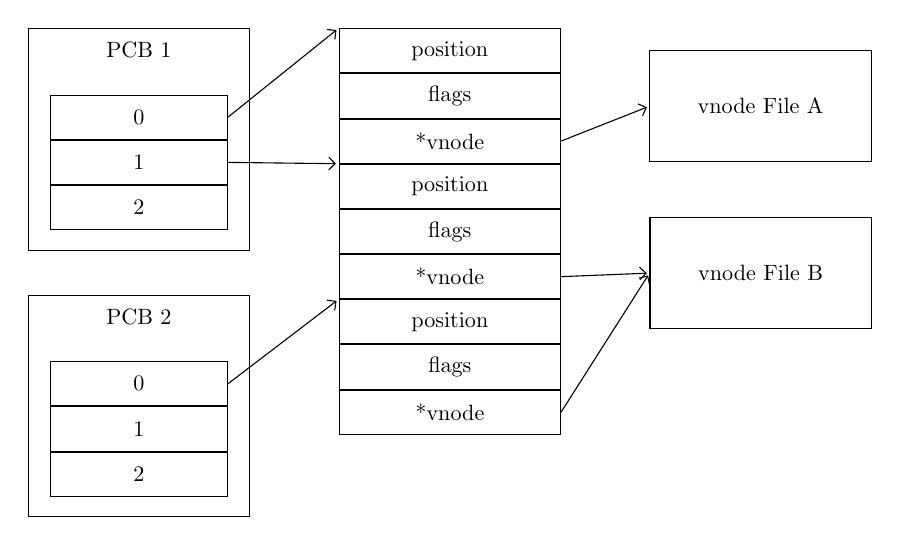
\begin{tikzpicture}[node distance=0mm and 0mm,scale=0.8, every node/.style={transform shape}]
      \node[rectangle,draw,minimum width=100,minimum height=100] (pcb1)      {};
      \node[rectangle,minimum width=100,minimum height=20,yshift=-20] (pcb11) [above=of pcb1] {PCB 1};
      \node[rectangle,draw,minimum width=80,minimum height=20,xshift=0,yshift=-10] (lof11) [below=of pcb11] {0};
      \node[rectangle,draw,minimum width=80,minimum height=20] (lof12) [below=of lof11] {1};
      \node[rectangle,draw,minimum width=80,minimum height=20] (lof13) [below=of lof12] {2};


      \node[rectangle,draw,minimum width=100,minimum height=100,yshift=-20] (pcb2)   [below=of pcb1]   {};
      \node[rectangle,minimum width=100,minimum height=20,yshift=-20] (pcb21) [above=of pcb2] {PCB 2};
      \node[rectangle,draw,minimum width=80,minimum height=20,xshift=0,yshift=-10] (lof21) [below=of pcb21] {0};
      \node[rectangle,draw,minimum width=80,minimum height=20] (lof22) [below=of lof21] {1};
      \node[rectangle,draw,minimum width=80,minimum height=20] (lof23) [below=of lof22] {2};

      \node[rectangle,draw,minimum width=100,minimum height=20,xshift=40,yshift=40] (gof1)   [right=of pcb1]   {position};
      \node[rectangle,draw,minimum width=100,minimum height=20] (gof2)   [below=of gof1]   {flags};
      \node[rectangle,draw,minimum width=100,minimum height=20] (gof3)   [below=of gof2]   {*vnode};

      \node[rectangle,draw,minimum width=100,minimum height=20] (gof4)   [below=of gof3]   {position};
      \node[rectangle,draw,minimum width=100,minimum height=20] (gof5)   [below=of gof4]   {flags};
      \node[rectangle,draw,minimum width=100,minimum height=20] (gof6)   [below=of gof5]   {*vnode};

      \node[rectangle,draw,minimum width=100,minimum height=20] (gof7)   [below=of gof6]   {position};
      \node[rectangle,draw,minimum width=100,minimum height=20] (gof8)   [below=of gof7]   {flags};
      \node[rectangle,draw,minimum width=100,minimum height=20] (gof9)   [below=of gof8]   {*vnode};

      \node[rectangle,draw,minimum width=100,minimum height=50,xshift=40,yshift=-25] (vnode1)  [right=of gof1]    {vnode File A};
      \node[rectangle,draw,minimum width=100,minimum height=50,yshift=-25] (vnode2)  [below=of vnode1]    {vnode File B};

      \draw[->] (lof11.east) -- (gof1.north west);
      \draw[->] (lof12.east) -- (gof4.north west);
      \draw[->] (lof21.east) -- (gof7.north west);

      \draw[->] (gof3.east) -- (vnode1.west);
      \draw[->] (gof6.east) -- (vnode2.west);
      \draw[->] (gof9.east) -- (vnode2.west);        
    \end{tikzpicture}
  \end{frame}

  \begin{frame}{Each Process Contains a File Table in its PCB}

    A File Descriptor is an index in the table

    \vspace{2em}

    Each item points to a system-wide \textit{global open file table}

    \vspace{2em}

    The GOF table holds information about the seek position and flags

    \hspace{2em} It also points to a \textit{VNode} (supports read/write/etc)

    \vspace{2em}

    A vnode (virtual mode) holds information about the file

    \hspace{2em} vnodes can represent regular files, pipes, network sockets, etc.
  \end{frame}

  \begin{frame}{Remember What Happens In A Fork}
     PCB is copied on fork

     \vspace{2em}

     Specifically for us, the local open file table gets inherited

     \vspace{2em}

     Both PCBs point to the same Global Open File Table entry
  \end{frame}

  \begin{frame}{Both Processes Point to the Same GOF Entry}
    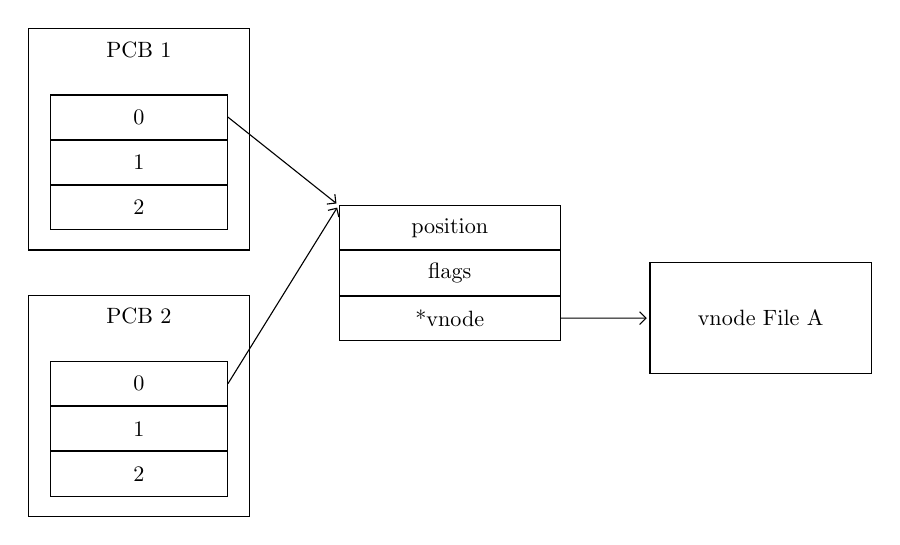
\begin{tikzpicture}[node distance=0mm and 0mm,scale=0.8, every node/.style={transform shape}]
      
      \node[rectangle,draw,minimum width=100,minimum height=100] (pcb1)      {};
      \node[rectangle,minimum width=100,minimum height=20,yshift=-20] (pcb11) [above=of pcb1] {PCB 1};
      \node[rectangle,draw,minimum width=80,minimum height=20,xshift=0,yshift=-10] (lof11) [below=of pcb11] {0};
      \node[rectangle,draw,minimum width=80,minimum height=20] (lof12) [below=of lof11] {1};
      \node[rectangle,draw,minimum width=80,minimum height=20] (lof13) [below=of lof12] {2};


      \node[rectangle,draw,minimum width=100,minimum height=100,yshift=-20] (pcb2)   [below=of pcb1]   {};
      \node[rectangle,minimum width=100,minimum height=20,yshift=-20] (pcb21) [above=of pcb2] {PCB 2};
      \node[rectangle,draw,minimum width=80,minimum height=20,xshift=0,yshift=-10] (lof21) [below=of pcb21] {0};
      \node[rectangle,draw,minimum width=80,minimum height=20] (lof22) [below=of lof21] {1};
      \node[rectangle,draw,minimum width=80,minimum height=20] (lof23) [below=of lof22] {2};

      \node[rectangle,draw,minimum width=100,minimum height=20,xshift=40,yshift=-40] (gof1)   [right=of pcb1]   {position};
      \node[rectangle,draw,minimum width=100,minimum height=20] (gof2)   [below=of gof1]   {flags};
      \node[rectangle,draw,minimum width=100,minimum height=20] (gof3)   [below=of gof2]   {*vnode};

      \node[rectangle,draw,minimum width=100,minimum height=50,xshift=40] (vnode1)  [right=of gof3]    {vnode File A};

      \draw[->] (lof11.east) -- (gof1.north west);
      \draw[->] (lof21.east) -- (gof1.north west);

      \draw[->] (gof3.east) -- (vnode1.west);    

    \end{tikzpicture}
  \end{frame}

  \begin{frame}{There Are Some ``Gotchas'' For This Sharing}
    Current position in file is shared between both processes

    \vspace{2em}

    Seek in one process leads to seek in all other processes using the same GOF entry

    \vspace{2em}

    Opening the same file in both processes after forking creates multiple
    GOF entries
  \end{frame}

  \begin{frame}[fragile]{How many LOF and GOF Entries Exist? What is the Relationship?}
    \begin{lstlisting}
open("todo.txt", O_RDONLY);
fork();
open("b.txt", O_RDONLY);
    \end{lstlisting}

    \vspace{2em}

    Assume there are no previously opened files (not even the standard ones)
  \end{frame}

  \begin{frame}{There are 2 LOF Entries Each, and 3 GOF Entries}

    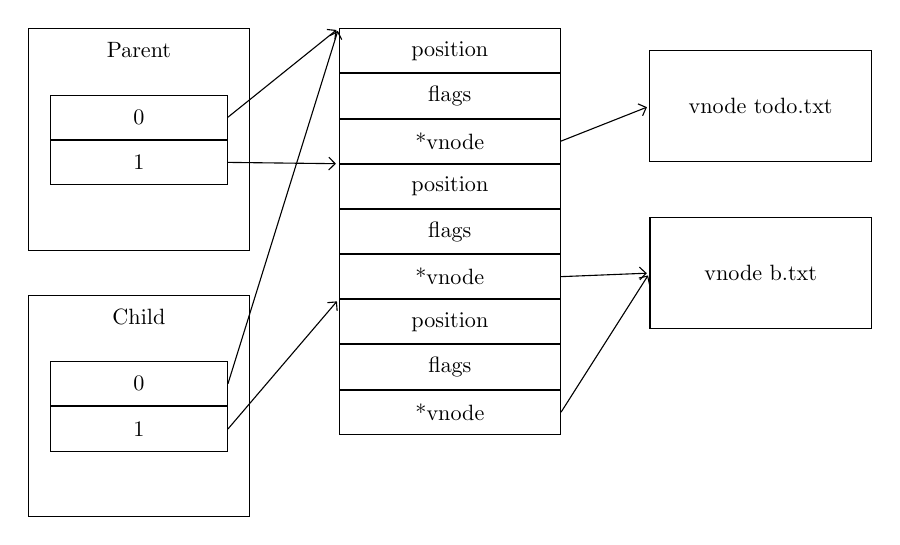
\begin{tikzpicture}[node distance=0mm and 0mm,scale=0.8, every node/.style={transform shape}]
        
      \node[rectangle,draw,minimum width=100,minimum height=100] (pcb1)      {};
      \node[rectangle,minimum width=100,minimum height=20,yshift=-20] (pcb11) [above=of pcb1] {Parent};
      \node[rectangle,draw,minimum width=80,minimum height=20,xshift=0,yshift=-10] (lof11) [below=of pcb11] {0};
      \node[rectangle,draw,minimum width=80,minimum height=20] (lof12) [below=of lof11] {1};


      \node[rectangle,draw,minimum width=100,minimum height=100,yshift=-20] (pcb2)   [below=of pcb1]   {};
      \node[rectangle,minimum width=100,minimum height=20,yshift=-20] (pcb21) [above=of pcb2] {Child};
      \node[rectangle,draw,minimum width=80,minimum height=20,xshift=0,yshift=-10] (lof21) [below=of pcb21] {0};
      \node[rectangle,draw,minimum width=80,minimum height=20] (lof22) [below=of lof21] {1};

      \node[rectangle,draw,minimum width=100,minimum height=20,xshift=40,yshift=40] (gof1)   [right=of pcb1]   {position};
      \node[rectangle,draw,minimum width=100,minimum height=20] (gof2)   [below=of gof1]   {flags};
      \node[rectangle,draw,minimum width=100,minimum height=20] (gof3)   [below=of gof2]   {*vnode};

      \node[rectangle,draw,minimum width=100,minimum height=20] (gof4)   [below=of gof3]   {position};
      \node[rectangle,draw,minimum width=100,minimum height=20] (gof5)   [below=of gof4]   {flags};
      \node[rectangle,draw,minimum width=100,minimum height=20] (gof6)   [below=of gof5]   {*vnode};

      \node[rectangle,draw,minimum width=100,minimum height=20] (gof7)   [below=of gof6]   {position};
      \node[rectangle,draw,minimum width=100,minimum height=20] (gof8)   [below=of gof7]   {flags};
      \node[rectangle,draw,minimum width=100,minimum height=20] (gof9)   [below=of gof8]   {*vnode};

      \node[rectangle,draw,minimum width=100,minimum height=50,xshift=40,yshift=-25] (vnode1)  [right=of gof1]    {vnode todo.txt};
      \node[rectangle,draw,minimum width=100,minimum height=50,yshift=-25] (vnode2)  [below=of vnode1]    {vnode b.txt};

      \draw[->] (lof11.east) -- (gof1.north west);
      \draw[->] (lof12.east) -- (gof4.north west);
      \draw[->] (lof21.east) -- (gof1.north west);
      \draw[->] (lof22.east) -- (gof7.north west);

      \draw[->] (gof3.east) -- (vnode1.west);
      \draw[->] (gof6.east) -- (vnode2.west);
      \draw[->] (gof9.east) -- (vnode2.west);        

    \end{tikzpicture}
  \end{frame}

  \begin{frame}{How Do We Store Files? Contiguous Allocation?}
    
    \begin{center}
        
      \begin{tikzpicture}[node distance=14mm and 14mm]

        \node[rectangle,draw,minimum width=30,minimum height=30,fill=solarizedgreen] (b1)   {};
        \node[rectangle,draw,minimum width=30,minimum height=30,fill=solarizedgreen] (b2) [right of=b1]  {};
        \node[rectangle,draw,minimum width=30,minimum height=30,fill=solarizedgreen] (b3) [right of=b2]  {};
        \node[rectangle,draw,minimum width=30,minimum height=30] (b4) [right of=b3]  {};
        \node[rectangle,draw,minimum width=30,minimum height=30] (b5) [right of=b4]  {};

        \node[rectangle,draw,minimum width=30,minimum height=30] (b6) [below of=b1]  {};
        \node[rectangle,draw,minimum width=30,minimum height=30,fill=solarizedred] (b7) [right of=b6]  {};
        \node[rectangle,draw,minimum width=30,minimum height=30,fill=solarizedred] (b8) [right of=b7]  {};
        \node[rectangle,draw,minimum width=30,minimum height=30,fill=solarizedred] (b9) [right of=b8]  {};
        \node[rectangle,draw,minimum width=30,minimum height=30,fill=solarizedred] (b10) [right of=b9]  {};

        \node[rectangle,draw,minimum width=30,minimum height=30,fill=solarizedred] (b11) [below of=b6]  {};
        \node[rectangle,draw,minimum width=30,minimum height=30,fill=solarizedred] (b12) [right of=b11]  {};
        \node[rectangle,draw,minimum width=30,minimum height=30,fill=solarizedblue] (b13) [right of=b12]  {};
        \node[rectangle,draw,minimum width=30,minimum height=30,fill=solarizedblue] (b14) [right of=b13]  {};
        \node[rectangle,draw,minimum width=30,minimum height=30,fill=solarizedblue] (b15) [right of=b14]  {};

        \node[rectangle,draw,minimum width=30,minimum height=30,fill=solarizedblue] (b16) [below of=b11]  {};
        \node[rectangle,draw,minimum width=30,minimum height=30] (b17) [right of=b16]  {};
        \node[rectangle,draw,minimum width=30,minimum height=30] (b18) [right of=b17]  {};
        \node[rectangle,draw,minimum width=30,minimum height=30] (b19) [right of=b18]  {};
        \node[rectangle,draw,minimum width=30,minimum height=30] (b20) [right of=b19]  {};

        \node[rectangle,draw,minimum width=30,minimum height=30] (b21) [below of=b16]  {};
        \node[rectangle,draw,minimum width=30,minimum height=30] (b22) [right of=b21]  {};
        \node[rectangle,draw,minimum width=30,minimum height=30] (b23) [right of=b22]  {};
        \node[rectangle,draw,minimum width=30,minimum height=30] (b24) [right of=b23]  {};
        \node[rectangle,draw,minimum width=30,minimum height=30] (b25) [right of=b24]  {};

      \end{tikzpicture}

    \end{center}
  \end{frame}

  \begin{frame}{Contiguous Allocation Is Fast, If There Are No Modifications}
    Space efficient: Only start block and \# of blocks need to be stored

    \vspace{2em}

    Fast random access: $block = floor(\frac{offset}{blocksize})$

    \vspace{2em}
    Files can not grow easily

    \hspace{2em} Internal fragmentation (may not fill a block)
    
    \hspace{2em} External fragmentation when files are deleted or truncated
  \end{frame}

  \begin{frame}{What About Storing Like a Free List of Pages? Linked Allocation}
    \begin{center}
      \begin{tikzpicture}[node distance=14mm and 14mm]

        \node[rectangle,draw,minimum width=30,minimum height=30,fill=solarizedgreen] (b1)   {};
        \node[rectangle,draw,minimum width=30,minimum height=30] (b2) [right of=b1]  {};
        \node[rectangle,draw,minimum width=30,minimum height=30,fill=solarizedgreen] (b3) [right of=b2]  {};
        \node[rectangle,draw,minimum width=30,minimum height=30] (b4) [right of=b3]  {};
        \node[rectangle,draw,minimum width=30,minimum height=30] (b5) [right of=b4]  {};

        \node[rectangle,draw,minimum width=30,minimum height=30] (b6) [below of=b1]  {};
        \node[rectangle,draw,minimum width=30,minimum height=30,fill=solarizedgreen] (b7) [right of=b6]  {};
        \node[rectangle,draw,minimum width=30,minimum height=30] (b8) [right of=b7]  {};
        \node[rectangle,draw,minimum width=30,minimum height=30] (b9) [right of=b8]  {};
        \node[rectangle,draw,minimum width=30,minimum height=30,fill=solarizedgreen] (b10) [right of=b9]  {};

        \node[rectangle,draw,minimum width=30,minimum height=30] (b11) [below of=b6]  {};
        \node[rectangle,draw,minimum width=30,minimum height=30] (b12) [right of=b11]  {};
        \node[rectangle,draw,minimum width=30,minimum height=30] (b13) [right of=b12]  {};
        \node[rectangle,draw,minimum width=30,minimum height=30,fill=solarizedgreen] (b14) [right of=b13]  {};
        \node[rectangle,draw,minimum width=30,minimum height=30] (b15) [right of=b14]  {};

        \node[rectangle,draw,minimum width=30,minimum height=30] (b16) [below of=b11]  {};
        \node[rectangle,draw,minimum width=30,minimum height=30] (b17) [right of=b16]  {};
        \node[rectangle,draw,minimum width=30,minimum height=30] (b18) [right of=b17]  {};
        \node[rectangle,draw,minimum width=30,minimum height=30,fill=solarizedgreen] (b19) [right of=b18]  {};
        \node[rectangle,draw,minimum width=30,minimum height=30] (b20) [right of=b19]  {};

        \node[rectangle,draw,minimum width=30,minimum height=30] (b21) [below of=b16]  {};
        \node[rectangle,draw,minimum width=30,minimum height=30] (b22) [right of=b21]  {};
        \node[rectangle,draw,minimum width=30,minimum height=30] (b23) [right of=b22]  {};
        \node[rectangle,draw,minimum width=30,minimum height=30] (b24) [right of=b23]  {};
        \node[rectangle,draw,minimum width=30,minimum height=30] (b25) [right of=b24]  {};

        \draw[->,line width=1mm,draw=solarizedblue] (b1.east) -- (b7.west);
        \draw[->,line width=1mm,draw=solarizedblue] (b7.east) -- (b3.west);
        \draw[->,line width=1mm,draw=solarizedblue] (b3.east) -- (b14.west);
        \draw[->,line width=1mm,draw=solarizedblue] (b14.east) -- (b10.west);
        \draw[->,line width=1mm,draw=solarizedblue] (b10.east) -- (b19.west);

      \end{tikzpicture}
    \end{center}
  \end{frame}

  \begin{frame}{Linked Allocation Has Slow Random Access}
    
    Space efficient: Only start block needs to be stored

    \hspace{2em} Blocks need to store a pointer to the next block (block is slightly smaller)

    \vspace{2em}

    Files can grow/shrink

    \hspace{2em} No external fragmentation

    \hspace{2em} Internal fragmentation

    \vspace{2em}

    How can we increase random access speed? We need to walk each block

    \hspace{2em} Each block may be located far away (it will never be cached)

  \end{frame}


  \begin{frame}{File Allocation Table Moves The List to a Separate Table}
    
    \begin{center}
        
      \begin{tikzpicture}[node distance=14mm and 14mm]

        \node[rectangle,draw,minimum width=30,minimum height=30,fill=solarizedgreen] (b1)   {0};
        \node[rectangle,draw,minimum width=30,minimum height=30] (b2) [right of=b1]  {1};
        \node[rectangle,draw,minimum width=30,minimum height=30,fill=solarizedgreen] (b3) [right of=b2]  {2};
        \node[rectangle,draw,minimum width=30,minimum height=30] (b4) [right of=b3]  {3};
        \node[rectangle,draw,minimum width=30,minimum height=30] (b5) [right of=b4]  {4};

        \node[rectangle,draw,minimum width=30,minimum height=30] (b6) [below of=b1]  {5};
        \node[rectangle,draw,minimum width=30,minimum height=30,fill=solarizedgreen] (b7) [right of=b6]  {6};
        \node[rectangle,draw,minimum width=30,minimum height=30] (b8) [right of=b7]  {7};
        \node[rectangle,draw,minimum width=30,minimum height=30] (b9) [right of=b8]  {8};
        \node[rectangle,draw,minimum width=30,minimum height=30,fill=solarizedgreen] (b10) [right of=b9]  {9};

        \node[rectangle,draw,minimum width=30,minimum height=30] (b11) [below of=b6]  {10};
        \node[rectangle,draw,minimum width=30,minimum height=30] (b12) [right of=b11]  {11};
        \node[rectangle,draw,minimum width=30,minimum height=30] (b13) [right of=b12]  {12};
        \node[rectangle,draw,minimum width=30,minimum height=30,fill=solarizedgreen] (b14) [right of=b13]  {13};
        \node[rectangle,draw,minimum width=30,minimum height=30] (b15) [right of=b14]  {14};

        \node[rectangle,draw,minimum width=30,minimum height=30] (b16) [below of=b11]  {15};
        \node[rectangle,draw,minimum width=30,minimum height=30] (b17) [right of=b16]  {16};
        \node[rectangle,draw,minimum width=30,minimum height=30] (b18) [right of=b17]  {17};
        \node[rectangle,draw,minimum width=30,minimum height=30,fill=solarizedgreen] (b19) [right of=b18]  {18};
        \node[rectangle,draw,minimum width=30,minimum height=30] (b20) [right of=b19]  {19};

        \node[rectangle,draw,minimum width=30,minimum height=30] (b21) [below of=b16]  {20};
        \node[rectangle,draw,minimum width=30,minimum height=30] (b22) [right of=b21]  {21};
        \node[rectangle,draw,minimum width=30,minimum height=30] (b23) [right of=b22]  {22};
        \node[rectangle,draw,minimum width=30,minimum height=30] (b24) [right of=b23]  {23};
        \node[rectangle,draw,minimum width=30,minimum height=30] (b25) [right of=b24]  {24};

        \node[rectangle,draw,minimum width=30,minimum height=10,xshift=-40,fill=solarizedgreen] (fat1) [left=of b1] {0};
        \node[rectangle,draw,minimum width=30,minimum height=10,yshift=40] (fat2) [below=of fat1] {1};
        \node[rectangle,draw,minimum width=30,minimum height=10,yshift=40,fill=solarizedgreen] (fat3) [below=of fat2] {2};
        \node[rectangle,draw,minimum width=30,minimum height=10,yshift=40] (fat4) [below=of fat3] {3};
        \node[rectangle,draw,minimum width=30,minimum height=10,yshift=40] (fat5) [below=of fat4] {4};
        \node[rectangle,draw,minimum width=30,minimum height=10,yshift=40] (fat6) [below=of fat5] {5};
        \node[rectangle,draw,minimum width=30,minimum height=10,yshift=40,fill=solarizedgreen] (fat7) [below=of fat6] {6};
        \node[rectangle,draw,minimum width=30,minimum height=10,yshift=40] (fat8) [below=of fat7] {7};
        \node[rectangle,draw,minimum width=30,minimum height=10,yshift=40] (fat9) [below=of fat8] {8};
        \node[rectangle,draw,minimum width=30,minimum height=10,yshift=40,fill=solarizedgreen] (fat10) [below=of fat9] {9};
        \node[rectangle,draw,minimum width=30,minimum height=10,yshift=40] (fat11) [below=of fat10] {10};
        \node[rectangle,draw,minimum width=30,minimum height=10,yshift=40] (fat12) [below=of fat11] {11};
        \node[rectangle,draw,minimum width=30,minimum height=10,yshift=40] (fat13) [below=of fat12] {12};

        \node[rectangle,draw,minimum width=30,minimum height=10,xshift=-20,fill=solarizedgreen] (fat14) [right=of fat1] {13};
        \node[rectangle,draw,minimum width=30,minimum height=10,yshift=40] (fat15) [below=of fat14] {14};

        \node[rectangle,draw,minimum width=30,minimum height=10,yshift=40] (fat16) [below=of fat15] {15};
        \node[rectangle,draw,minimum width=30,minimum height=10,yshift=40] (fat17) [below=of fat16] {16};
        \node[rectangle,draw,minimum width=30,minimum height=10,yshift=40] (fat18) [below=of fat17] {17};
        \node[rectangle,draw,minimum width=30,minimum height=10,yshift=40,fill=solarizedgreen] (fat19) [below=of fat18] {18};
        \node[rectangle,draw,minimum width=30,minimum height=10,yshift=40] (fat20) [below=of fat19] {19};
        \node[rectangle,draw,minimum width=30,minimum height=10,yshift=40] (fat21) [below=of fat20] {20};
        \node[rectangle,draw,minimum width=30,minimum height=10,yshift=40] (fat22) [below=of fat21] {21};
        \node[rectangle,draw,minimum width=30,minimum height=10,yshift=40] (fat23) [below=of fat22] {22};
        \node[rectangle,draw,minimum width=30,minimum height=10,yshift=40] (fat24) [below=of fat23] {23};
        \node[rectangle,draw,minimum width=30,minimum height=10,yshift=40] (fat25) [below=of fat24] {24};

        \draw[->,line width=1mm,color=solarizedblue] (fat1.west) -- (fat7.west);
        \draw[->,line width=1mm,color=solarizedblue] (fat7.east) -- (fat3.east);
        \draw[->,line width=1mm,color=solarizedblue] (fat3.east) -- (fat14.west);
        \draw[->,line width=1mm,color=solarizedblue] (fat14.east) -- (fat10.west);
        \draw[->,line width=1mm,color=solarizedblue] (fat10.east) -- (fat19.west);

      \end{tikzpicture}

    \end{center}
  \end{frame}

  \begin{frame}{File Allocation Table (FAT) is Similar to Linked Allocation}
    Files can grow/shrink

    \hspace{2em} No external fragmentation

    \hspace{2em} Internal fragmentation

    \vspace{2em}

    Fast random access: FAT can be held in memory/cache
    
    \hspace{2em} FAT size is linear to disk size: can become very large

    \vspace{2em}

    How can we further increase random access speed?
  \end{frame}

  \begin{frame}{Indexed Allocation Maps Each Block Directly}
    \begin{center}
      \begin{tikzpicture}[node distance=14mm and 14mm]

        \node[rectangle,draw,minimum width=30,minimum height=30,fill=solarizedgreen] (b1)   {};
        \node[rectangle,draw,minimum width=30,minimum height=30] (b2) [right of=b1]  {};
        \node[rectangle,draw,minimum width=30,minimum height=30,fill=solarizedgreen] (b3) [right of=b2]  {};
        \node[rectangle,draw,minimum width=30,minimum height=30] (b4) [right of=b3]  {};
        \node[rectangle,draw,minimum width=30,minimum height=30] (b5) [right of=b4]  {};

        \node[rectangle,draw,minimum width=30,minimum height=30] (b6) [below of=b1]  {};
        \node[rectangle,draw,minimum width=30,minimum height=30,fill=solarizedgreen] (b7) [right of=b6]  {};
        \node[rectangle,draw,minimum width=30,minimum height=30] (b8) [right of=b7]  {};
        \node[rectangle,draw,minimum width=30,minimum height=30] (b9) [right of=b8]  {};
        \node[rectangle,draw,minimum width=30,minimum height=30,fill=solarizedgreen] (b10) [right of=b9]  {};

        \node[rectangle,draw,minimum width=30,minimum height=30,fill=solarizedred] (b11) [below of=b6]  {};
        \node[rectangle,draw,minimum width=30,minimum height=30] (b12) [right of=b11]  {};
        \node[rectangle,draw,minimum width=30,minimum height=30] (b13) [right of=b12]  {};
        \node[rectangle,draw,minimum width=30,minimum height=30,fill=solarizedgreen] (b14) [right of=b13]  {};
        \node[rectangle,draw,minimum width=30,minimum height=30] (b15) [right of=b14]  {};

        \node[rectangle,draw,minimum width=30,minimum height=30] (b16) [below of=b11]  {};
        \node[rectangle,draw,minimum width=30,minimum height=30] (b17) [right of=b16]  {};
        \node[rectangle,draw,minimum width=30,minimum height=30] (b18) [right of=b17]  {};
        \node[rectangle,draw,minimum width=30,minimum height=30,fill=solarizedgreen] (b19) [right of=b18]  {};
        \node[rectangle,draw,minimum width=30,minimum height=30] (b20) [right of=b19]  {};

        \node[rectangle,draw,minimum width=30,minimum height=30] (b21) [below of=b16]  {};
        \node[rectangle,draw,minimum width=30,minimum height=30] (b22) [right of=b21]  {};
        \node[rectangle,draw,minimum width=30,minimum height=30] (b23) [right of=b22]  {};
        \node[rectangle,draw,minimum width=30,minimum height=30] (b24) [right of=b23]  {};
        \node[rectangle,draw,minimum width=30,minimum height=30] (b25) [right of=b24]  {};

        \node[rectangle,draw,minimum width=80,minimum height=170,xshift=-50] (index) [left of=b11]  {};
        \node[rectangle,draw,minimum width=60,minimum height=20,yshift=-70] (index1) [above=of index] {Block 0};
        \node[rectangle,draw,minimum width=60,minimum height=20,yshift=34] (index2) [below=of index1] {Block 1};
        \node[rectangle,draw,minimum width=60,minimum height=20,yshift=34] (index3) [below=of index2] {Block 2};
        \node[rectangle,draw,minimum width=60,minimum height=20,yshift=34] (index4) [below=of index3] {Block 3};
        \node[rectangle,draw,minimum width=60,minimum height=20,yshift=34] (index5) [below=of index4] {Block 4};
        \node[rectangle,draw,minimum width=60,minimum height=20,yshift=34] (index6) [below=of index5] {Block 5};

        \draw[-] (index.north east) -- (b11.north west);
        \draw[-] (index.south east) -- (b11.south west);

        \draw[->,line width=0.5mm,color=solarizedblue] (index1.east) -- (b1.west);
        \draw[->,line width=0.5mm,color=solarizedblue] (index2.east) -- (b7.west);
        \draw[->,line width=0.5mm,color=solarizedblue] (index3.east) -- (b3.west);
        \draw[->,line width=0.5mm,color=solarizedblue] (index4.east) -- (b14.west);
        \draw[->,line width=0.5mm,color=solarizedblue] (index5.east) -- (b10.west);
        \draw[->,line width=0.5mm,color=solarizedblue] (index6.east) -- (b19.west);

      \end{tikzpicture}
    \end{center}
  \end{frame}

  \begin{frame}{For Indexed Allocation, Each File Needs an Index Block}
    Files can still grow/shrink

    \hspace{2em} No external fragmentation

    \hspace{2em} Internal fragmentation

    \vspace{2em}

    Fast random access

    \vspace{2em}

    File size limited by the maximum size of the index block (fit it in one block)
  \end{frame}

  \begin{frame}{Indexed Allocation Problem}
    
    Assume this scenario:
    \begin{itemize}
      \item An index block stores pointers to data blocks only (no meta information)
      \item A disk block is 8~KiB in size
      \item A pointer to a block is 4~Bytes
    \end{itemize}

    \vspace{2em}

    What is the maximum size of a file managed by this index block?
  \end{frame}

  \begin{frame}{Indexed Allocation Solution}
    
    Assume this scenario:
    \begin{itemize}
      \item An index block stores pointers to data blocks only (no meta information)
      \item A disk block is 8~KiB in size
      \item A pointer to a block is 4~Bytes
    \end{itemize}

    \vspace{2em}

    \# of pointers = $\mathsf{\frac{8 KiB}{4 B} \frac{2^{13} B}{2^2 B} = 2^{11}}$

    \# of addressable blocks = \# of pointers

    Total of bytes = $\mathsf{2^{11} \times 2^{13} = 2^{24} = 16 MiB}$
  \end{frame}

  \begin{frame}{An inode Describes a File System Object (Files and Directories)}
    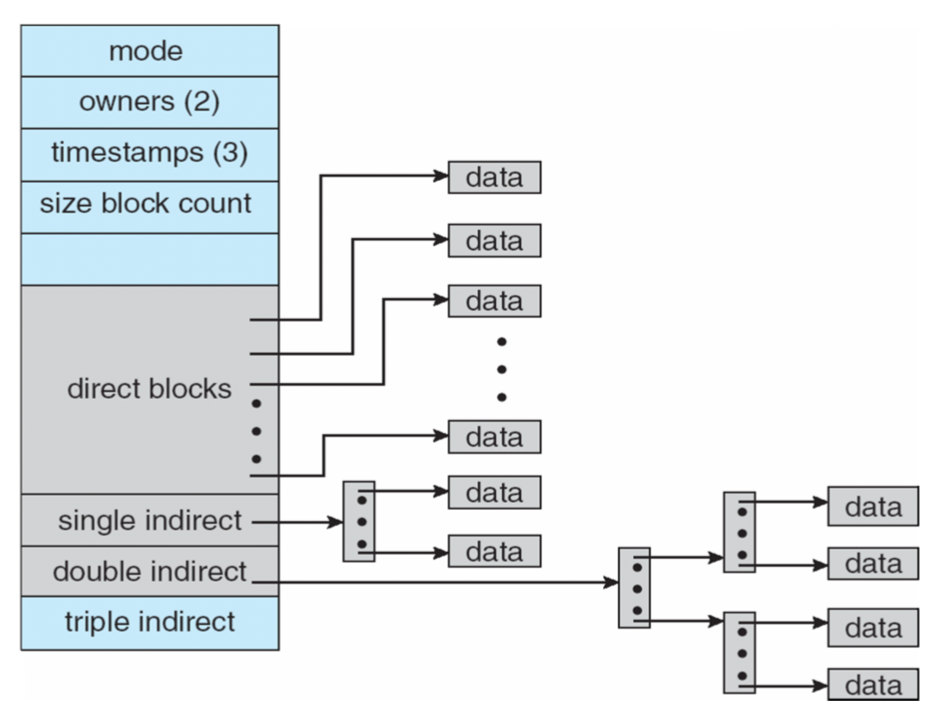
\includegraphics[height=0.8\textheight]{hinode.png}
  \end{frame}

  \begin{frame}{Linux inodes Aim to Be Efficient for Small Files, and Support Large Ones}
    UNIX inodes hold metadata and pointers to blocks

    \vspace{2em}

    Smaller files only use direct pointers

    \vspace{2em}

    Larger files have additional index nodes with pointers to additional blocks

    \vspace{2em}

    Very small files can have it's contents directly inside the inode
  \end{frame}

  \begin{frame}{inode Problem}
    
    Assume this scenario:
    \begin{itemize}
      \item An index block stores 12 direct pointers, 1 single, double and triple indirect pointer each
      \item A disk block is 8~KiB in size
      \item A pointer to a block is 4~Bytes
      \item Indirect blocks consist of direct pointers only
    \end{itemize}


    \vspace{2em}

    What is the maximum size of a file managed by this index block?
  \end{frame}

  \begin{frame}{inode Solution}
    
    Assume this scenario:
    \begin{itemize}
      \item An index block stores 12 direct pointers, 1 single, double and triple indirect pointer each
      \item A disk block is 8~KiB in size
      \item A pointer to a block is 4~Bytes
      \item Indirect blocks consist of direct pointers only
    \end{itemize}

    \vspace{2em}

    \# pointers per indirect table = $\mathsf{\frac{2^{13}}{2^2} = 2^{11}}$

    \# addressable blocks = $\mathsf{12 + 2^{11} + (2^{11})^2 + (2^{11})^3 \approx (2^{11})^3 = 2^{33}}$

    Total of bytes = $\mathsf{2^{33} * 2^{13} = 2^{46} = 64 TiB}$
  \end{frame}

  \begin{frame}{Hard Links Are Pointers to inodes}

    \begin{center}
      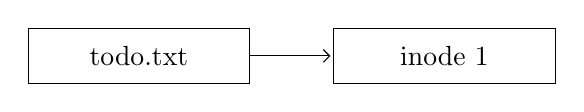
\begin{tikzpicture}[node distance=0mm and 0mm]

        \node[rectangle,draw,minimum width=80,minimum height=20] (inode1)   {inode 1};
        \node[rectangle,draw,minimum width=80,minimum height=20,xshift=-30] (fileA)  [left=of inode1] {todo.txt};

        \draw[->] (fileA.east) -- (inode1.west);

      \end{tikzpicture}

    \end{center}

    A directory entry (aka filename) is called a \textit{hard link}

    \vspace{2em}

    A hard link points to one inode
  \end{frame}

  \begin{frame}{Multiple Hard Links Can Point to the Same inode}

    \begin{center}
        
      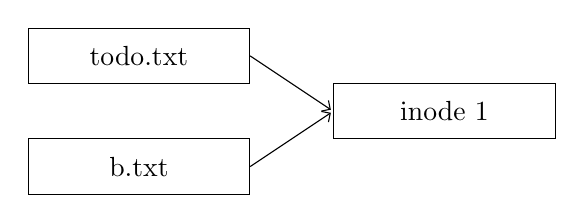
\begin{tikzpicture}[node distance=0mm and 0mm]

        \node[rectangle,draw,minimum width=80,minimum height=20] (inode1)   {inode 1};
        \node[rectangle,draw,minimum width=80,minimum height=20,xshift=-30,yshift=20] (fileA)  [left=of inode1] {todo.txt};
        \node[rectangle,draw,minimum width=80,minimum height=20,xshift=-30,yshift=-20] (fileB)  [left=of inode1] {b.txt};

        \draw[->] (fileA.east) -- (inode1.west);
        \draw[->] (fileB.east) -- (inode1.west);

      \end{tikzpicture}

    \end{center}

    Deleting a file only removes a hard link (the file can be hard liked somewhere else)

    \vspace{2em}

    POSIX has the \texttt{unlink} call rather than a delete call
  \end{frame}

  \begin{frame}{Soft Links Are Paths to Another File}

    \begin{center}
        
      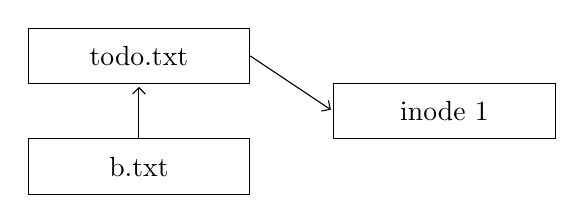
\begin{tikzpicture}[node distance=0mm and 0mm]

        \node[rectangle,draw,minimum width=80,minimum height=20] (inode1)   {inode 1};
        \node[rectangle,draw,minimum width=80,minimum height=20,xshift=-30,yshift=20] (fileA)  [left=of inode1] {todo.txt};
        \node[rectangle,draw,minimum width=80,minimum height=20,xshift=-30,yshift=-20] (fileB)  [left=of inode1] {b.txt};

        \draw[->] (fileA.east) -- (inode1.west);
        \draw[->] (fileB.north) -- (fileA.south);

      \end{tikzpicture}

    \end{center}

    When resolving the file, the file system is redirected somewhere else, so:
    \begin{itemize}
      \item Soft link targets do not need to exist
      \item Soft link targets can be deleted without notice of the soft link
      \item Unresolvable soft links lead to an exception
    \end{itemize}
  \end{frame}

  \begin{frame}[fragile]{Filesystem Example Problem}
    \begin{lstlisting}
touch todo.txt
ln todo.txt b.txt
ln -s todo.txt c.txt
mv todo.txt d.txt
rm b.txt
    \end{lstlisting}

    \vspace{2em}

    How does the FS look like before and after the mv and rm commands?
  \end{frame}


  \begin{frame}[fragile]{Filesystem Example Solution (1)}
    \begin{lstlisting}
touch todo.txt
ln todo.txt b.txt
ln -s todo.txt c.txt
mv todo.txt d.txt
rm b.txt
    \end{lstlisting}

    Before mv:
    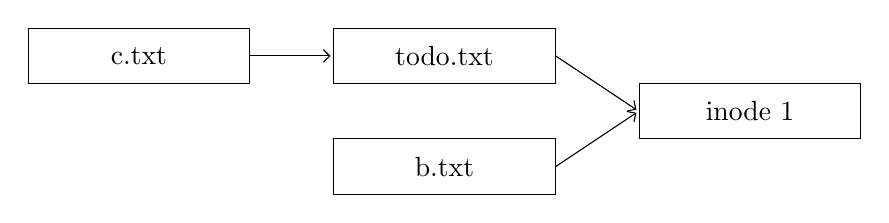
\begin{tikzpicture}[node distance=0mm and 0mm]

      \node[rectangle,draw,minimum width=80,minimum height=20] (inode1)   {inode 1};
      \node[rectangle,draw,minimum width=80,minimum height=20,xshift=-30,yshift=20] (fileA)  [left=of inode1] {todo.txt};
      \node[rectangle,draw,minimum width=80,minimum height=20,xshift=-30,yshift=-20] (fileB)  [left=of inode1] {b.txt};
      \node[rectangle,draw,minimum width=80,minimum height=20,xshift=-30] (fileC)  [left=of fileA] {c.txt};
  
      \draw[->] (fileA.east) -- (inode1.west);
      \draw[->] (fileB.east) -- (inode1.west);
      \draw[->] (fileC.east) -- (fileA.west);
    
    \end{tikzpicture}

  \end{frame}

  \begin{frame}[fragile]{Filesystem Example Solution (2)}
    \begin{lstlisting}
touch todo.txt
ln todo.txt b.txt
ln -s todo.txt c.txt
mv todo.txt d.txt
rm b.txt
    \end{lstlisting}

    After mv:
    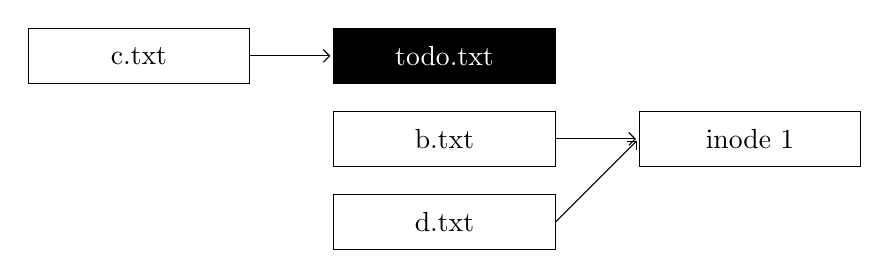
\begin{tikzpicture}[node distance=0mm and 0mm]

      \node[rectangle,draw,minimum width=80,minimum height=20] (inode1)   {inode 1};
      \node[rectangle,draw,minimum width=80,minimum height=20,xshift=-30,yshift=30,fill=black,text=white] (fileA)  [left=of inode1] {todo.txt};
      \node[rectangle,draw,minimum width=80,minimum height=20,xshift=-30] (fileB)  [left=of inode1] {b.txt};
      \node[rectangle,draw,minimum width=80,minimum height=20,xshift=-30,yshift=-30] (fileD)  [left=of inode1] {d.txt};
      \node[rectangle,draw,minimum width=80,minimum height=20,xshift=-30] (fileC)  [left=of fileA] {c.txt};
  
      \draw[->] (fileD.east) -- (inode1.west);
      \draw[->] (fileB.east) -- (inode1.west);
      \draw[->] (fileC.east) -- (fileA.west);
    
    \end{tikzpicture}

  \end{frame}

  \begin{frame}[fragile]{Filesystem Example Solution (3)}
    \begin{lstlisting}
touch todo.txt
ln todo.txt b.txt
ln -s todo.txt c.txt
mv todo.txt d.txt
rm b.txt
    \end{lstlisting}

    After rm:\\\,\\
    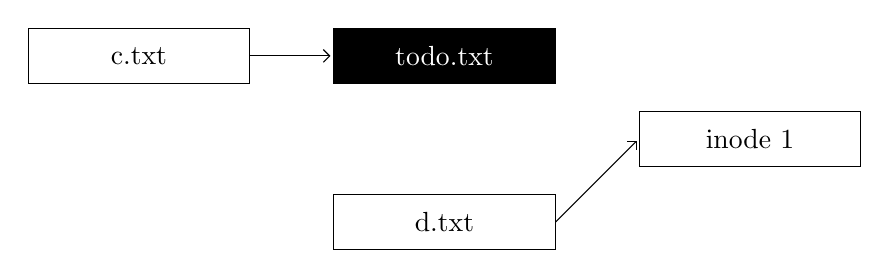
\begin{tikzpicture}[node distance=0mm and 0mm]

      \node[rectangle,draw,minimum width=80,minimum height=20] (inode1)   {inode 1};
      \node[rectangle,draw,minimum width=80,minimum height=20,xshift=-30,yshift=30,fill=black,text=white] (fileA)  [left=of inode1] {todo.txt};
      \node[rectangle,draw,minimum width=80,minimum height=20,xshift=-30,yshift=-30] (fileD)  [left=of inode1] {d.txt};
      \node[rectangle,draw,minimum width=80,minimum height=20,xshift=-30] (fileC)  [left=of fileA] {c.txt};
    
      \draw[->] (fileD.east) -- (inode1.west);
      \draw[->] (fileC.east) -- (fileA.west);
    
    \end{tikzpicture}

  \end{frame}

  \begin{frame}{In UNIX, Everything is a File}
    Directories are files of type ``directory''

    \vspace{2em}

    Additional types are ``regular file'', ``block device'' (HDDs, SSDs), ``pipe'', ``socket'' etc.

    \vspace{2em}

    Directory inodes do not store pointers to data blocks but rather filenames and pointers to inodes
  \end{frame}

  \begin{frame}{What Data is Stored in an inode?}
     \small
      \begin{itemize}
        \item[a] Filename
        \item[b] Containing Directory name
        \item[c] File Size 
        \item[d] File type
        \item[e] \# of soft links to file
        \item[f] location of soft links 
        \item[g] \# of hard links to file  
        \item[h] location of hard links
        \item[i] access rights
        \item[j] timestamps
        \item[k] file contents
        \item[l] ordered list of data blocks     
      \end{itemize}
  \end{frame}

  \begin{frame}{What Data is Stored in an inode? Solution}
     \small
      \begin{itemize}
        \item[a] Filename \textit{No. Names are stored in directories}
        \item[b] Containing Directory name \textit{No. File can be in multiple dirs}
        \item[c] File Size \textit{Yes}
        \item[d] File type \textit{Yes}
        \item[e] \# of soft links to file \textit{No (they are unknown)}
        \item[f] location of soft links \textit{No (they are unknown)}
        \item[g] \# of hard links to file \textit{Yes (to know when to erase the file, check \texttt{stat})}
        \item[h] location of hard links \textit{No (they are unknown to the inode)}
        \item[i] access rights \textit{Yes}
        \item[j] timestamps \textit{Yes}
        \item[k] file contents \textit{Sometimes}
        \item[l] ordered list of data blocks \textit{Yes, by definition} 
      \end{itemize}
  \end{frame}

  \begin{frame}{Filesystem Caches Speed Up Writing to Disks}

    Writing data to the disk is slow, we can use a cache to speed it up

    \vspace{2em}

    File blocks are cached in main memory in the \textit{filesystem cache}
    
    \hspace{2em} Referenced blocks are likely to be referenced again (temporal locality)

    \hspace{2em}Logically near blocks are likely to be referenced (spatial locality)

    \vspace{2em}

    A kernel thread (or daemon) writes changes periodically to disk

    \vspace{2em}
    
    \texttt{flush} and \texttt{sync} system calls trigger a permanent write
  \end{frame}

  \begin{frame}{Journaling Filesystem}
    Deleting a file on a Unix file system involves three steps:

    \begin{enumerate}
      \item Removing its directory entry.
      \item Releasing the inode to the pool of free inodes.
      \item Returning all disk blocks to the pool of free disk blocks.
    \end{enumerate}

    \vspace{2em}

    Crashes could occur between any steps, leading to a storage leak

    \vspace{2em}

    The journal contains operations in progress, so if a crash occurs we can recover
  \end{frame}


  \begin{frame}{Filesystems Enable Persistence}
    They describe how files are stored on disks:
    \begin{itemize}
      \item API-wise you can open files, and change the position to read/write
            at
      \item Each process has a local open file and there's a global open file
            table
      \item There's multiple allocation strategies: contiguous, linked, FAT, indexed
      \item Linux uses a hybrid inode approach
      \item Everything is a file on UNIX, names in a directory can be hard or soft links
      
    \end{itemize}
  \end{frame}
\end{document}
